% Komponentendiagramm des Projektes
\section{Komponentendiagramm}

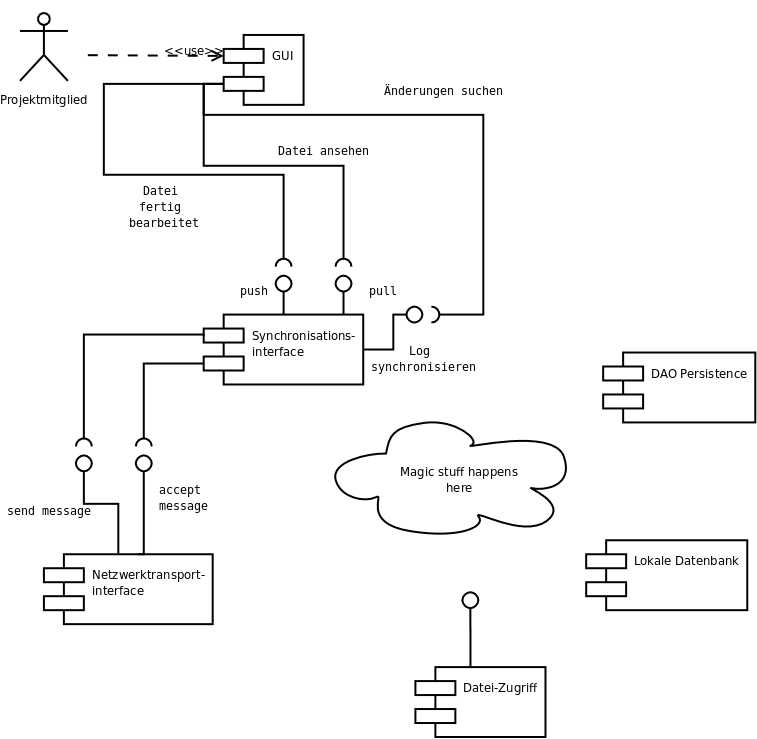
\includegraphics[width=0.98\textwidth]{../uml/component_diagram.png}

Das Projekt ist in 6 Komponenten aufgeteilt. 
\begin{itemize}
	\item Core
	\item Graphical User Interface (GUI)
	\item Database Persistence (DAO)
	\item Synchronisation Services
	\item File System Services
	\item Network Service
\end{itemize}

% Wie man sieht habe ich sehr viel dazugeschrieben. Allgemein ist mein Verständnis von einer Komponente das, dass ich von ihr wissen will, wofür ich sie nutzen kann und was sie mir für Services anbietet. ~simon

% Es sollen zuerst die Aufgaben jeder Komponente beschrieben.
% Danach kann auf Verbindung zu anderen Komponenten eingegangen werden.

\subsection{Core}
In der Core-Komponente befindet sich die Business Logic der Applikation. Hier werden die Abläufe bei bestimmten User-Eingaben (z.B. das Drücken des Buttons ``Synchronisieren"), mit Hilfe der einzelnen Komponenten, durchgeführt. 
Der Core reagiert aber auch auf Events, die durch die einzelnen Komponenten gemeldet werden, z.B. wenn eine Datei im Dateisystem geändert wird, wird dies an den Core gemeldet. Dieser steuert die GUI und und je nach User Interaktion wird die Kontrolle wieder zurückgegeben. 

\subsection{Graphical User Interface}
Das Graphical User Interface (GUI) ist die grafische Benutzeroberfläche, mit welcher der Endanwender arbeitet.
Die GUI ermöglicht Zugriff auf alle von der ``Core"-Komponente für Endbenutzer zur Verfügung gestellten
Funktionalitäten.

% Persistence NICHT Database Persistence, es ist nicht festgelegt dass wir eine Datenbank verwenden ~simon
\subsection{Persistence} 
Die Persistence Komponente abstrahiert den Zugriff auf die Daten, die für den Betrieb gespeichert werden müssen. Diese umschließen nicht die Dateien. Es wird das Konzept des Data Hiding umgesetzt, wodurch erreicht werden kann, dass die anderen Komponenten nur auf definierte Weise die Daten verwenden. Für die Speicherung der Daten kann eine relationale Datenbank verwendet werden.

\subsection{Synchronisation Services}
Die Synchronisationskomponente ist für die Verteilung von Änderungensinformationen und Dateninhalten an andere
Projektmitglieder/Clients zuständig. 

\subsection{File System Services}
Die File System Services kapselt den Zugriff auf Dateien im Dateisystem. Außerdem kann diese Komponente durch
entsprechende Strategien feststellen, ob Dateien geändert wurden oder in die Projektordnerstruktur kopiert wurden und dies dem Core mitteilen, welcher wiederum entsprechende Aktionen veranlasst.

\subsection{Interclient Communication} 
Der Interclient Communication Service kapselt die vollständige Kommunikation zwischen den Clients (über das Netzwerk) und gibt die entsprechenden Nachrichten an den Core weiter. So ist es leicht möglich, verschiedene Netzwerkbackends (z.B. XMPP oder RMI) zu unterstützen, welche für den Core und somit für den Benutzer transparent sind. Außerdem wird die Authentifizierung der
Nutzer in dieser Komponente durchgeführt. 
% Ich habe bei Client Authentifizierung ein schlechtes Gefühl. Wenn wir nicht mit XMPP arbeiten, wie werden die Clients dann Authentifiziert?
% ja. ~johannes

